\part{Teoretická část}

\chapter{Asymptotická notace}

\section{O-notace}
Odkaz v závorekách: \cite[see][page 900]{einstein}\\
Odkaz: \cite{knuthwebsite}\\
A odkaz pod čarou: \footcite[see][s. 42]{latexcompanion}\\
Dobrý den, ahoj, \gls{xr}\\
$3.14 = \pi$

\section{Abeceda Abeceda Abeceda Abeceda Abeceda Abeceda Abeceda Abeceda Abeceda Abeceda }
\begin{figure}
    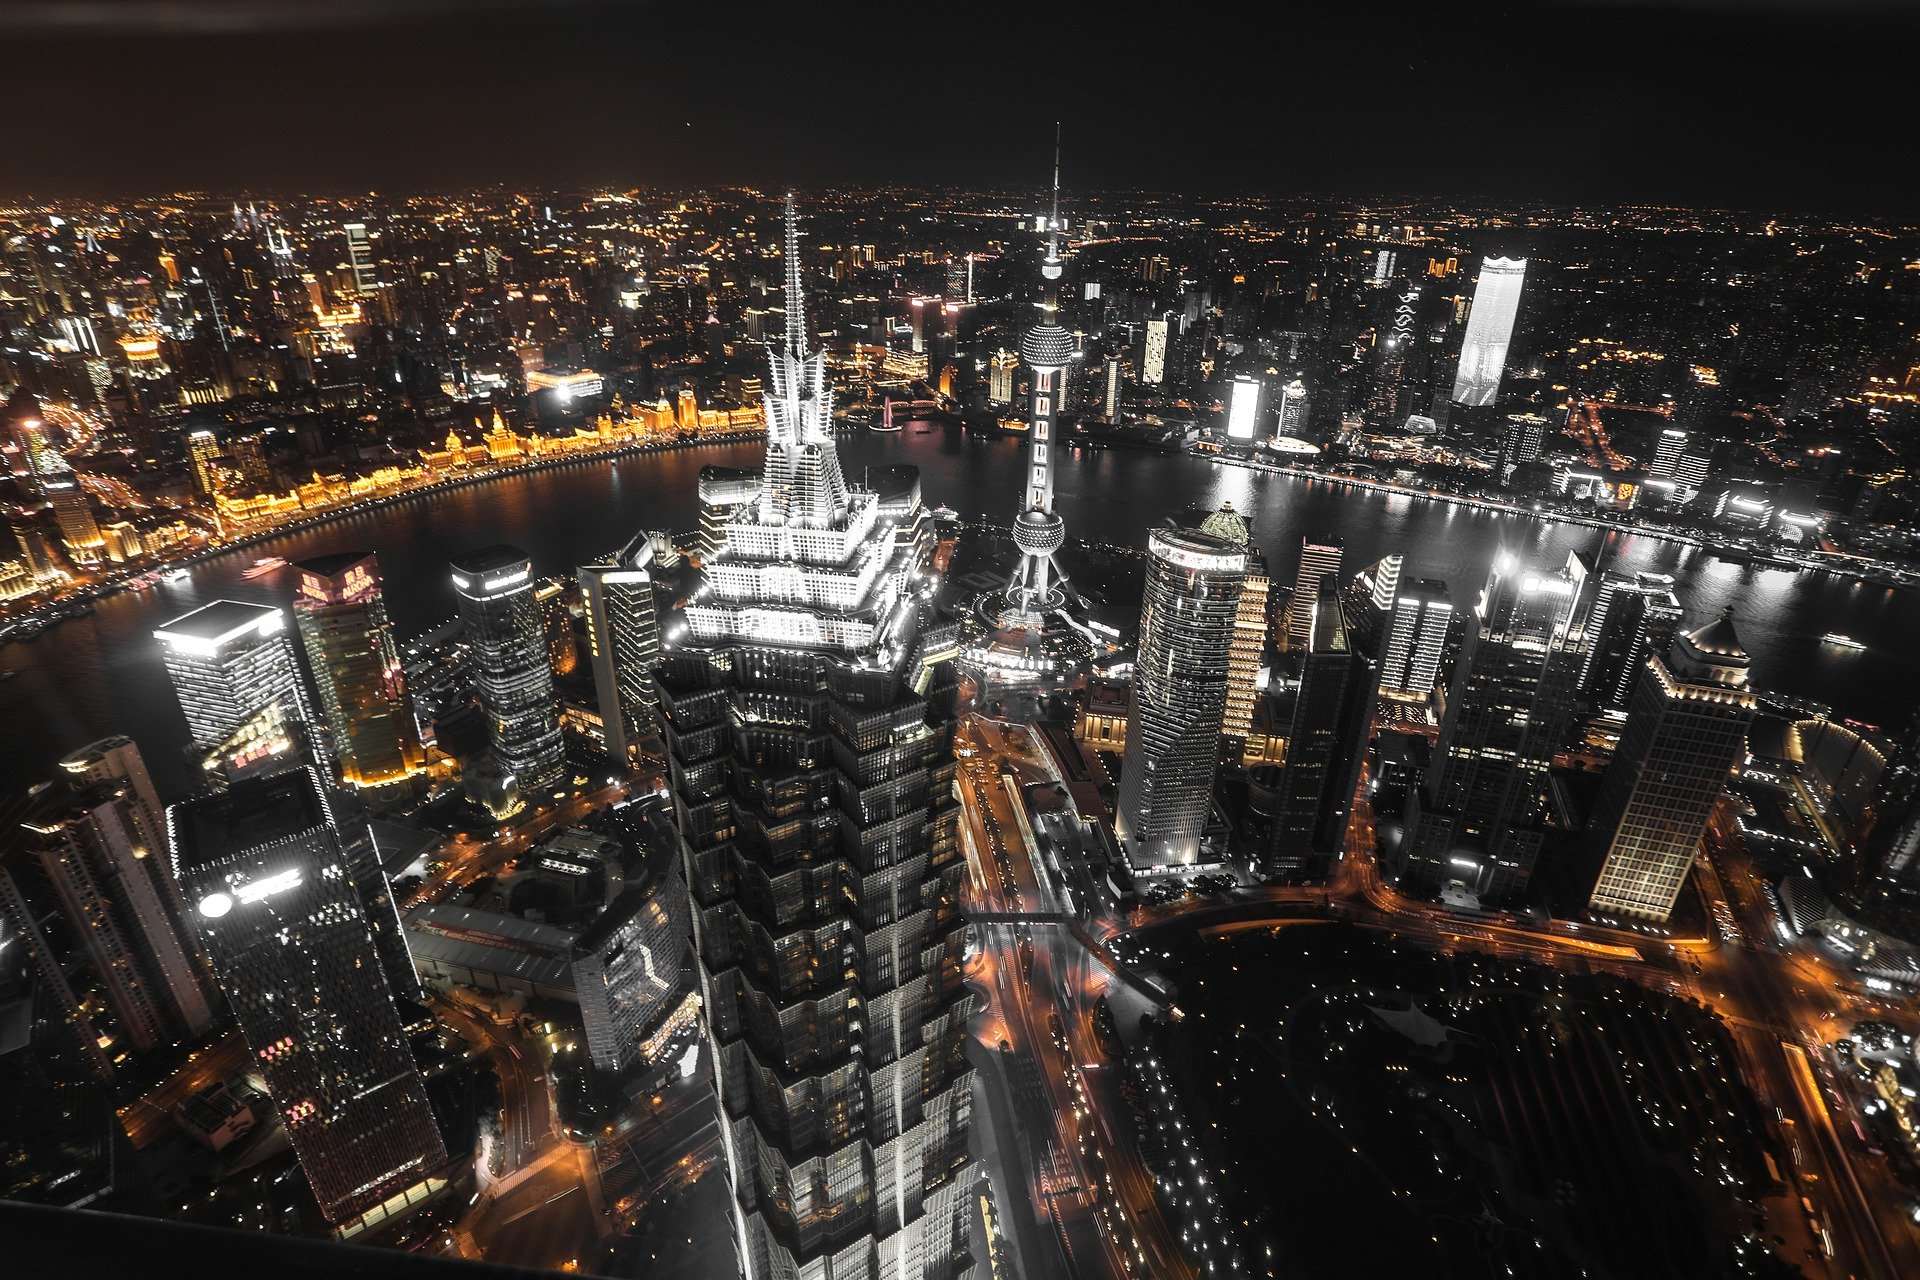
\includegraphics[width=\linewidth]{test.jpg}
    \caption{Testovací}
    \label{fig:test}
\end{figure}
\begin{table}
    \caption{Testovací}
    \label{tab:test2}
    \begin{tabular}{ccccc}
        1 & 1 & 1  & 1  & 1  \\
        1 & 2 & 3  & 4  & 5  \\
        1 & 3 & 6  & 10 & 15 \\
        1 & 4 & 10 & 30 & 45
    \end{tabular}
\end{table}

Obrázek \ref{fig:test} ukazuje Shangai z Pixabay.\\
Tabulka \ref{tab:test2} ukazuje hádejte, co.\\
Rovnice \ref{quad_eq} řeší kvadratickou rovnici.